\documentclass[a4paper,11pt]{article}

\usepackage[utf8]{inputenc}
\usepackage{lmodern}
\usepackage[english]{babel}
\usepackage[cm]{fullpage}
\usepackage[margin=2.5cm]{geometry}
\usepackage{multirow}
\usepackage{amsmath}
\usepackage{enumitem}
\usepackage[bookmarks]{hyperref}
\usepackage{ifthen}
\usepackage{fontspec}
\usepackage{graphicx}
\usepackage{fancyhdr}

\usepackage{tabularx}
\usepackage[table]{xcolor}
\usepackage{pdflscape}
\usepackage{multicol}

\graphicspath{{logos}{figures}}

\setmainfont[Ligatures=TeX]{DejaVu Sans}
\setsansfont[Ligatures=TeX]{DejaVu Sans}

\renewcommand{\familydefault}{\sfdefault}

\title{}
\author{}
\date{\today}
\pagestyle{empty}

\hypersetup
{
    pdfauthor={},
    pdftitle={eCSE Proposal},
    colorlinks={true},
    urlcolor={blue},
}
\urlstyle{same}

\pagestyle{fancy}
\setlength{\topmargin}{-3.5cm}
\setlength{\headheight}{2.5cm}
\setlength{\headsep}{0.5cm}
\lhead{\hspace{-5em}
\includegraphics[width=4cm]{epcc_logo.png}}
\chead{
\includegraphics[width=5cm]{ed_logo.png}\hspace{2em}
\includegraphics[width=4cm]{archer2_logo.png}}
\rhead{
\includegraphics[width=4cm]{ukri_logo.png}\hspace{-5em}}
\renewcommand{\headrulewidth}{0pt}
\cfoot{}

%\newcommand{\sect}[1]{\section{#1}}
%\newcommand{\ssect}[1]{\vspace{-0.5em}\subsection*{#1}\vspace{-0.5em}}
%\newcommand{\hrules}{\vspace{1pt}\hrule\vspace{2pt}}
%{\renewcommand{\arraystretch}{1.1}

\let\OLDthebibliography\thebibliography
\renewcommand\thebibliography[1]{
  \OLDthebibliography{#1}
  \setlength{\parskip}{0pt}
  \setlength{\itemsep}{0pt plus 0.3ex}
}

% Ensure you are using XeLaTeX to compile this document!
\begin{document}
\begin{center}
\huge \textbf{Proposal for a GPU eCSE Application}\\
\end{center}
Applicants for a \textbf{GPU eCSE application} should use this template.\\

\noindent This GPU eCSE call will close at \textbf{16:00 on Tuesday 19 March 2024}. No applications will be accepted after this time.\\

\noindent Please note:
\begin{itemize}[nosep]
	\item There is a hard page limit for each section which is shown at the start of each section. 
	\item The font size should be no smaller than 11pt and the margins should be no smaller than 2.5cm. 
\end{itemize}\vspace{1em}

\noindent Please upload your proposal when you fill in your eCSE application online form via the eCSE Funding Calls section within the SAFE: \url{https://safe.epcc.ed.ac.uk/}.\\

\noindent Please read the Applications Guidance (linked in to the page \url{https://www.archer2.ac.uk/ecse/calls/}) for further instructions on how to complete your eCSE online application.\\

\noindent If you have any queries or require assistance regarding your application, please contact the ARCHER2 service desk: \url{support@archer2.ac.uk}.

\section{Project Title (as given in on-line SAFE form)}
Firedrake: Code generation targeting GPU architectures

\section{PI Name and Institution}
David Ham\\
Imperial College London

\clearpage
\section{Description of code(s) (max. 2 page)}
Firedrake (\url{firedrakeproject.org}) is a high-level, high-productivity Python based system for the specification and solution of PDEs using the finite element method.
Parallelism is currently achieved through MPI.
Through the course of this eCSE we will transform proof of concept GPU functionality into a fully integrated capability, enabling GPU and MPI + GPU parallelism paradigms. 

The Firedrake framework itself consists of several Python packages and compiled scientific libraries, which are tightly integrated with one another to enable end users to express and solve continuum mechanics problems in ways that simply are not possible with other frameworks.
The Firedrake user base consists of hundreds if not thousands of UK and global individuals and is active use by leading research institutions such as UKAEA and the UK MetOffice, as well as many universities. 

Firedrake is almost entirely written in Python, as is pyop3; the underpinning domain-specific language (DSL) for the parallel executions of computational kernels on unstructured meshes.
The pyop3 layer alongside Loopy2, a loop optimisation framework, is responsible for generating and compiling efficient C kernels, which are executed to assemble the finite element operator.
These assembled operators are then passed to PETSc3 and the entire solver stack can be fully programmed through parameters. 

Firedrake also directly integrates with other well established scientific libraries installed as PETSc external packages, such as the HDF5 data format library, PTScotch partitioner, MUMPS and SuperLU\_dist parallel direct solvers, and hypre algebraic multigrid library. An installation of the whole Firedrake stack can be performed using a standard HPC toolchain of a compiler, MPI, and standard system libraries. 

Currently proof of concept GPU functionality for the entire Firedrake stack has been demonstrated using pyop3's predecessor, PyOP2.
The work of Kaushik Kulkarni[REF], ensures that the functionality we require of Loopy is already present upstream.
Furthermore, the Loopy team is happy to integrate future code to add additional functionality. 

Firedrake is already a well-established software framework on CPU, full functionality including advanced features, like geometric multigrid, hybridisation and patch preconditioning, is detailed in the user manual1 and on the website.
Firedrake is already the core of many downstream dependencies, such as Gusto, Thetis, Icepack to name a few.
As a result, Firedrake is already in use on the AMD Zen2 portion of ARCHER2 and has been since first becoming available to users in 2021.
The install procedure has been improved significantly as a result of eCSE04-5, where the Firedrake installation was adapted for the Spack installer and Singularity containers.
A containerised solution produced a ``zero install'' route to running Firedrake on ARCHER2 and has been successfully deployed on other systems since. 

Performance and scalability are both demonstrated in the paper ``Code generation for productive, portable, and scalable finite element simulation in Firedrake''4 and the numerical scaling data is summarised in the figures below for a test case on Isambard and ARCHER2. 

Many of the performance improvements to Firedrake in recent years have been a result of the work by the named technical staff.
Connor Ward has made countless improvements in transitioning from PyOP2 to pyop3, as well as adding a flamegraph profiler to PETSc which can be used to perform in depth performance analysis of small-scale Firedrake simulations.
Jack Betteridge is responsible for large scale HPC performance and stability improvements, which includes the addition of the necessary garbage collection routines required to run at extremely large scale (ie: exascale).

\begin{figure}
    \centering
    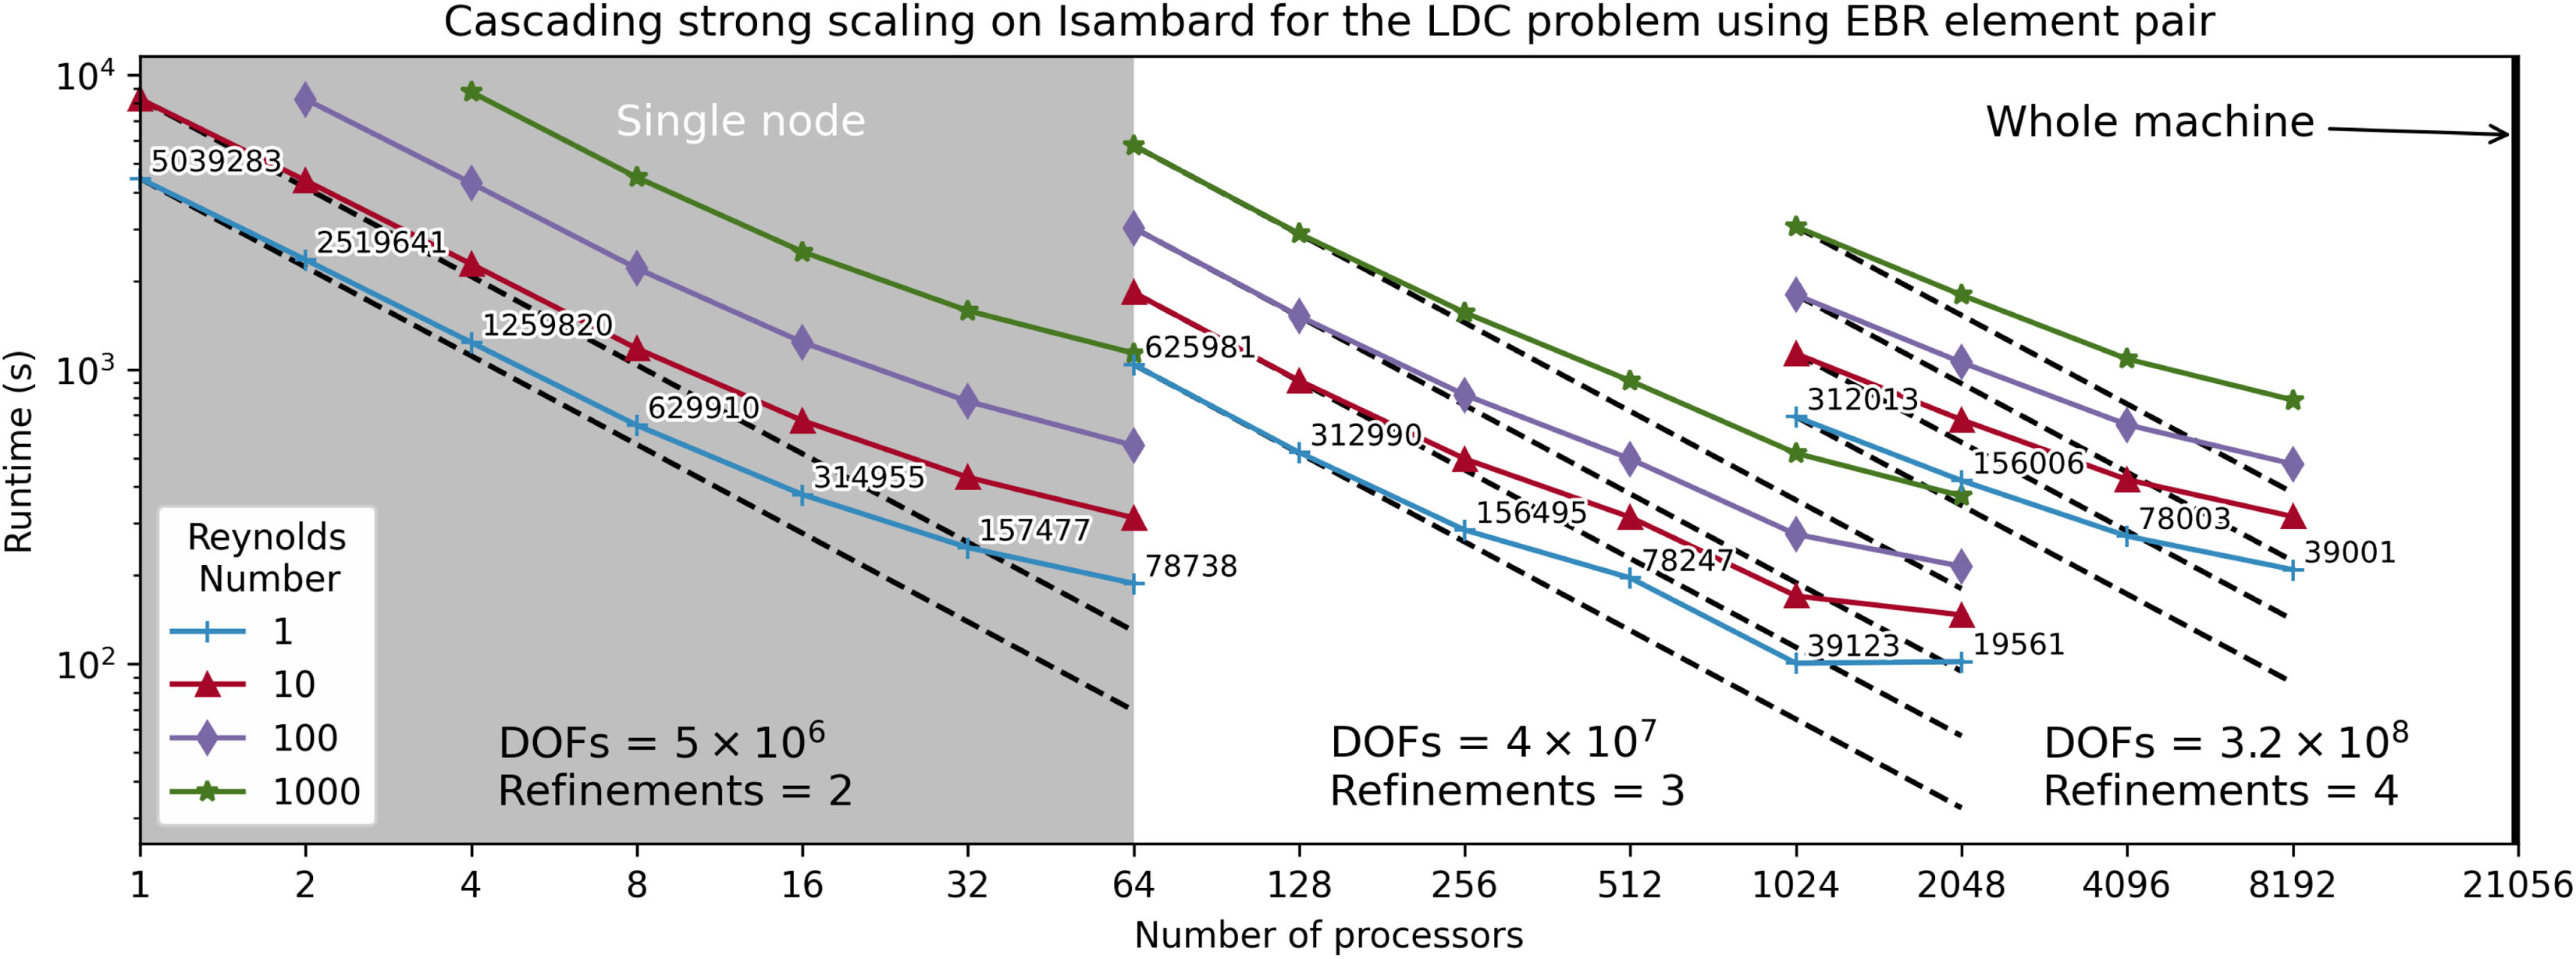
\includegraphics[width=\textwidth]{isambard.png}
    \caption{Strong scaling on Isambard}
\end{figure}

\begin{figure}
	\centering
	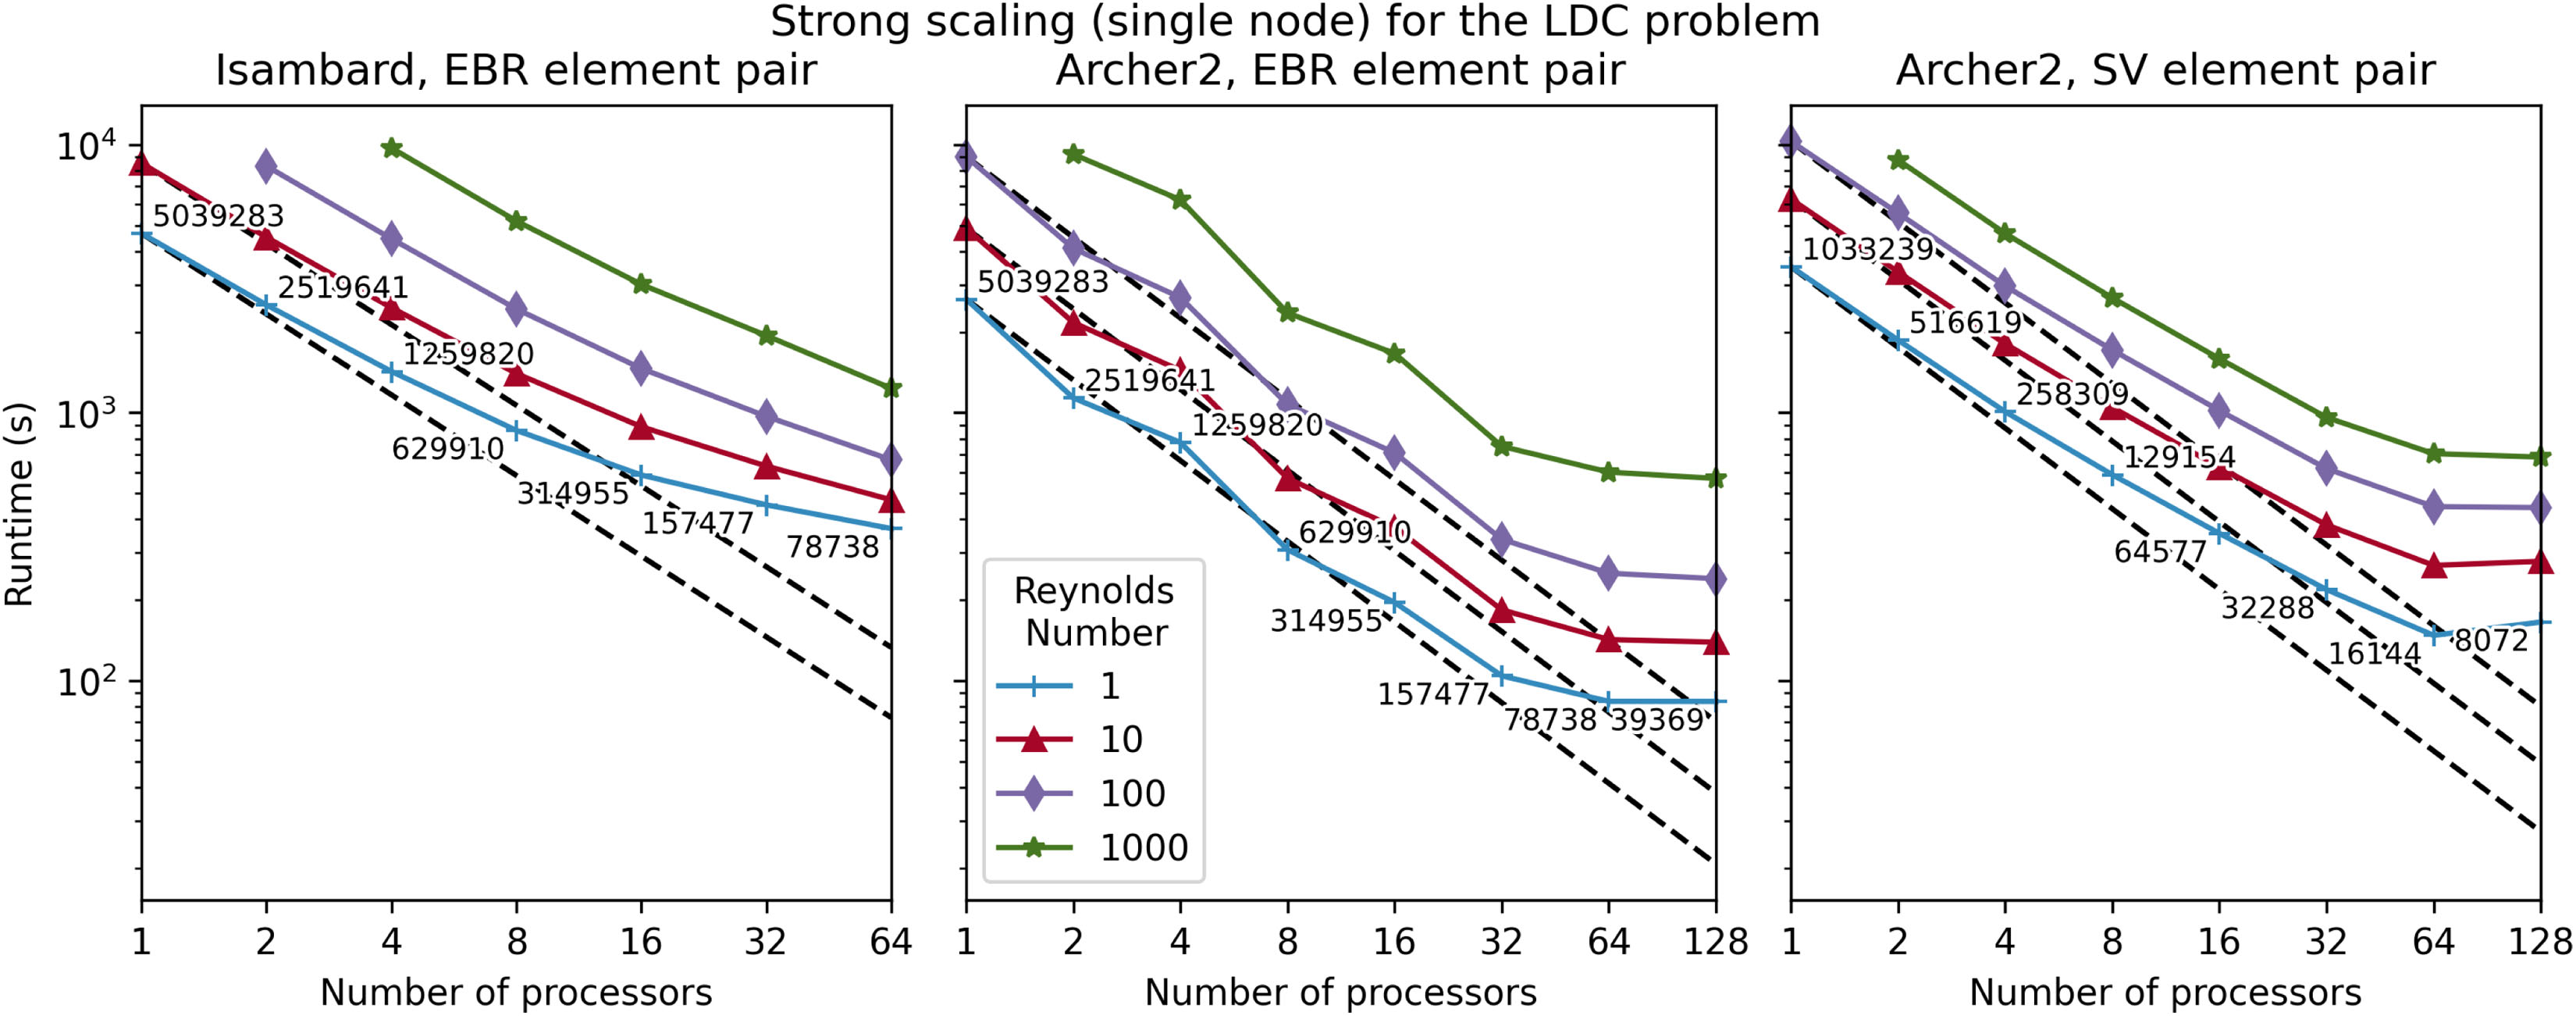
\includegraphics[width=\textwidth]{archer2.png}
	\caption{Scaling comparison}
\end{figure}


\clearpage
\section{Project Objectives and success metrics (max. 1 page)}
\noindent\textbf{WP1:}

\noindent\textbf{WP2:} A GPU-capable pyop3 library. pyop3 should be able to generate code for at least one, and preferably more, GPU backends (e.g. CUDA, OpenCL). At the same time pyop3 will also need to be able to coordinate data movement between CPU and GPU to avoid unnecessary copies.

The pyop3 repository will contain a considerable number of GPU tests that will be tested frequently under continuous integration for all supported backends. 

\noindent\textbf{WP3:} Firedrake can solve matrix-free problems using a GPU. 

The Firedrake test suite will include a number of tests validating that matrix-free solves of a variety of PDEs pass. 

\noindent\textbf{WP4:} Firedrake can solve matrix-explicit problems on a GPU. This is more challenging than the matrix-free case because it requires the integration of GPU-compatible sparse matrix assembly. 

The Firedrake test suite will include tests validating that matrix-explicit PDE solves work on GPU devices. 

\noindent\textbf{WP5:} Reimplement existing Firedrake preconditioners to work with GPUs. Priority will be given to patch preconditioners but other complex preconditioners like SLATE (static condensation and hybridisation) will be reimplemented if possible. 

The Firedrake test suite will include tests validating that these preconditioners yield the expected result and convergence rate on GPUs. 

\noindent\textbf{WP6:} Firedrake will have excellent weak- and strong-scaling performance on GPU-enabled nodes of ARCHER2. 
	
\noindent\textbf{WP7:}


\clearpage
\section{Project Overview, Technical Information and Workplan (max. 2 pages)}
The current state-of-the-art method for solving the equations of Magneto-Hydro Dynamics (MHD) and Computational Fluid Dynamics (CFD) problems is to use a multigrid approach.
Three key components of a robust solver are geometric multigrid, using matrix free methods and combining this with a patch smoother.
Geometric multigrid is used as a preconditioner over a hierarchy of meshes to achieve algorithmically optimal convergence, by reducing residual error at all scales.
Matrix-free methods allow more efficient memory use by never assembling the sparse matrix explicitly, but instead by applying the action of an operator and using iterative solvers.
Patch smoothers work by solving small problems in local regions of the solutions space, and a \emph{general} implementation is unique to Firedrake.
This is because constructing the operators for the patches requires information about the finite element space used in the discretisation, something just not possible when only using a sparse linear algebra library.
One also needs to be discerning in their choice of finite elements, a suitable combination will preserve quantities of interest by applying theory from Finite Element Exterior Calculus (FEEC). 

Firedrake, through its coupling with PETSc and sophisticated code generation for finite elements, is one of only a few frameworks with the capabilities to implement such solves.
However, these capabilities currently only exist on CPUs because: 
\begin{itemize}
	\item Firedrake’s finite element assembly code is only capable of targeting CPUs, and
	\item Due to the large amount of effort required in porting code to GPUs, only a few preconditioners in PETSc are available. In particular, the patch-based smoothers necessary for MHD/CFD applications are not implemented.
\end{itemize}
In this application, we are therefore proposing to tackle both of these shortcomings and make optimal solvers on GPUs a reality. 

\subsection{Technical information}
Adding GPU capabilities for MHD/CFD in Firedrake consists of two tasks: 
\begin{itemize}
	\item Enabling finite element assembly to take place on GPUs, and 
	\item Developing GPU-compatible preconditioners.
\end{itemize}
Critical to the accomplishing of both tasks is the development of one of Firedrake’s dependent libraries: pyop3. pyop3 is a new domain-specific language and code generator for expressing the application of computational kernels over unstructured meshes.
It was introduced to address shortcomings with its predecessor PyOP2 (cite).
In particular, pyop3 can describe a greater variety of loop expressions, which enables it to generate code for operators such as the patch preconditioners needed for fast MHD/CFD solvers.
In this proposal, we therefore seek to develop pyop3 to enable its code generator to target GPU architectures, and to use it to reimplement existing preconditioners such that they can target GPUs. 

An important point to stress is that we are not proposing ``porting'' code to GPUs.
Since Firedrake makes extensive use of code generation the intention is instead to modify the target architecture for the generated code and to make appropriate optimisations in our compiler toolchain.
This approach means that: 
\begin{itemize}
	\item The changes to Firedrake’s codebase will be contained to specific code-generation layers, and hence more maintainable.
	\item The changes will be compatible and composable with the rest of the Firedrake framework. For example, as a consequence of this work users will be able to run GPU-capable adjoint simulations with only a single-line change to their code.
\end{itemize}
This proposal will build on existing work as much as possible. A proof-of-concept code generation pipeline for GPUs has already been implemented in PyOP2 (Kulkarni, 2021), and extensive work has already been done to prepare PETSc for GPUs on exascale (Mills et al., 2020).

\begin{landscape}
\noindent\begin{tabularx}{1.49\textwidth}{|c|c|c|c|c|c|c|c|c|c|c|c|c|c|c|c|c|c|c|c|c|c|c|c|c|c|c|c|c|c|c|c|c}
\hline
Year & 24 &&&& 25 &&&&&&&&&&&& 26 &&&&&&&\\
Month &
09 & 10 & 11 & 12 &
01 & 02 & 03 & 04 & 05 & 06 & 07 & 08 & 09 & 10 & 11 & 12 &
01 & 02 & 03 & 04 & 05 & 06 & 07 & 08 \\\hline
JB & \multicolumn{2}{l|}{\cellcolor{orange}WP1} & \multicolumn{12}{l|}{\cellcolor{gray}} & \multicolumn{10}{l|}{\cellcolor{orange}WP6} \\\hline 
CW & \cellcolor{gray} & \multicolumn{5}{l|}{\cellcolor{orange}WP2} & \multicolumn{8}{l|}{\cellcolor{gray}} & \multicolumn{10}{l|}{\cellcolor{orange}WP7} \\\hline
CW & \multicolumn{4}{l|}{\cellcolor{gray}} & \multicolumn{6}{l|}{\cellcolor{orange}WP3} & \multicolumn{14}{l|}{\cellcolor{gray}} \\\hline
CW & \multicolumn{8}{l|}{\cellcolor{gray}} & \multicolumn{6}{l|}{\cellcolor{orange}WP4} & \multicolumn{10}{l|}{\cellcolor{gray}} \\\hline
CW & \multicolumn{12}{l|}{\cellcolor{gray}} & \multicolumn{6}{l|}{\cellcolor{orange}WP5} & \multicolumn{6}{l|}{\cellcolor{gray}} \\\hline
\end{tabularx}

\begin{multicols}{2}
In the first month of the grant, J. Betteridge will set up a GPU-ready Firedrake installation on ARCHER2. Once this is done, and having just completed his thesis on pyop3, C. Ward will take over the work and spend 11 months enabling GPU capabilities in Firedrake. In order, this work will roughly consist of: 
\begin{itemize}[itemsep=-2pt,topsep=2pt]
	\item Generate GPU code in pyop3.
    \item Matrix-free assembly in Firedrake. 
    \item Matrix-explicit assembly in Firedrake. 
    \item Develop GPU-compatible preconditioners. 
\end{itemize}

Once this work is complete, J.B. will rejoin the project and both staff will collaborate in a client-provider format: J.B. will test the code and run scaling experiments on ARCHER2, and C.W. will make bug fixes and performance improvements as they are discovered. This way we hope to ensure a GPU-compatible Firedrake that is robust and performant. 
%\columnbreak

\begin{tabularx}{\columnwidth}{|p{3cm}|X|}
\hline
Member of technical staff leaves the project (Low) &
Both technical staff will have frequent meetings such that they can pick up the other’s work and rapidly upskill potential replacement staff.
Good programming practices such as version control, continuous integration and code documentation will be used to reduce technical debt and facilitate others “picking up” the code. \\
\hline
pyop3 GPU capabilities take longer to implement than expected (Low) &
The other member of technical staff can step in and assist in the code development.\\
\hline
A particular feature cannot be implemented within the given timeframe (Medium) &
A version of Firedrake that provides an almost complete GPU-compatible feature set is still valuable to a large number of users.\\
\hline
\end{tabularx}
\end{multicols}
\end{landscape}


\clearpage
\section{Sustainability, maintenance, validation and {{availability}} of codes (max. 1 page)}
The Firedrake project is a completely open source project distributed under the GNU LGPL licence and has been publicly available online since 2013.
All development as part of this eCSE will take place in branches of existing public Firedrake repository or associated subpackages (\url{github.com/firedrakeproject}), which allows us to harness the existing testing and continuous integration (CI) framework already established by the project. 

Ongoing Firedrake development is part of an active research program at Imperial (David A. Ham) and Oxford (P. Farrell), with further contributions from many other UK and international institutions. Present support includes the following EPSRC projects: EP/W026163/1, EP/W026066/1 and EP/W029731/1. 

Maintenance is performed by a core team of developers, with additional contributions from other members of the community. The current CI ensures that: 
\begin{itemize}
	\item code is correctly formatted and linted,
	\item relevant documentation is present and can be built and displayed as a website,
	\item that all functionality tests pass,
	\item Firedrake containers are updated and released when code is incorporated into the main branch.
\end{itemize}
In addition to the above procedures, the core Firedrake team is improving coding standards within the project by documenting coding policies and procedures on the Firedrake wiki page.
Through this we will improve the consistency of code quality, whilst simultaneously providing a concrete reference to make it easier for collaborators to contribute. 

Present and future maintenance and support for using Firedrake is available through issues and discussions on GitHub, an active Slack channel with approximately 600 members, as well as a mailing list.
Firedrake also celebrates a high citation rate, the original Firedrake paper1 [CITE] and the recently published Firedrake Manual2 combined receive approximately 100 citations per year.
An active developer community ensures the longevity of any new functionality added by this eCSE. 

Since we will fully incorporate GPU functionality into Firedrake, anyone wishing to run the code developed in this programme will be able to.
During development users may checkout early solutions using the already existing development installation procedure.
After incorporating GPU functionality into the main Firedrake branch users will also enjoy the convenience of versioned containerised Firedrake images. 

To initially validate the new functionality of Firedrake running on GPUs, we will use dedicated workstations already available to the development team as well as the GPU portion of ARCHER2 to test scalability.
To integrate GPU validation into our CI it will be necessary to set up additional CI runners that have GPUs. Such machines are already present and available for use within the mathematics department at Imperial College London.
We will also update, verify and document the installation procedure specifically for ARCHER2.
1. F. Rathgeber et al., Firedrake: Automating the finite element method by composing abstractions, ACM Trans. Math. Softw., 2016

\clearpage
\section{Impact and Benefits (max. 1 page)}
Our project will expand the capabilities of Firedrake on any platform with a GPU available as an offload device.
This functionality will allow our present users to unlock new capabilities on machines that they already have Firedrake running on and install on many new exascale contenders.
One example would be current Firedrake ARCHER2 users, who will gain access to GPU capabilities by updating their existing installations.
Additionally, there are many tier 2 and tier 3 HPC Firedrake users who can currently only utilise the CPUs available on the machine, but who in the future will be able to harness the compute power and efficiency of GPUs too. 

A range of EPSRC/NERC grants support Firedrake and derived projects, with applications developed in the UK including coastal engineering (Thetis), numerical weather prediction (Gusto), and shape optimisation (Fireshape).
Firedrake is also used in many international software projects; geophysical modelling (g-adopt from the Australian National University and STMI from Universidade de São Paulo), glacier modelling (Icepack from University of Washington, USA), and timestepping (Irksome from Baylor University).
Enabling GPU capabilities in Firedrake will provide exciting new solutions for these existing teams, as well as spawning new research projects extending their current work to GPUs.
Firedrake is also used for developing cutting edge numerical methods, exciting new algorithmic possibilities will become available with the advent of GPU and hybrid CPU/GPU solvers and preconditioners.
Additionally, UKAEA and the UK MetOffice, two public sector research establishments with high priority use cases within the ExCALIBUR programme, are Firedrake users.
GPU functionality in Firedrake would allow simulations to be run on a UK based exascale machine, which will almost certainly require the use of accelerators to achieve exaFLOP performance

Firedrake already has range of tutorials demonstrating functionality, which are delivered multiple times per year to groups of current and prospective users both around the UK and overseas.
We anticipate that these tutorials will be portable to GPUs and an additional tutorial detailing the process will be created.
Tutorials will increase user awareness of the Firedrake framework and ease the transition required to move simulations from a laptop or desktop with a GPU to a HPC facility such as ARCHER2.

To further disseminate the benefits of this eCSE we intend to present the results of the eCSE at the large international SIAM Parallel Processing conference in early 2026.
Updates on progress and new functionality will be provided annually at the Firedrake Users meeting that is well attended by UK and international Firedrake users and developers.
In addition to the eCSE report, we will run a Firedrake tutorial as part of the ARCHER2 training programme as we have successfully done in the past. 

\end{document}
